%\documentclass[a4paper]{article}
\usepackage[utf8]{inputenc}
\usepackage[spanish, es-tabla, es-noshorthands]{babel}
\usepackage[table,xcdraw]{xcolor}
\usepackage[a4paper, footnotesep = 1cm, width=20cm, top=2.5cm, height=25cm, textwidth=18cm, textheight=25cm]{geometry}
%\geometry{showframe}

\usepackage{tikz}
\usepackage{amsmath}
\usepackage{amsfonts}
\usepackage{amssymb}
\usepackage{float}
\usepackage{graphicx}
\usepackage{caption}
\usepackage{subcaption}
\usepackage{multicol}
\usepackage{multirow}
\setlength{\doublerulesep}{\arrayrulewidth}
\usepackage{booktabs}
\usepackage{mathrsfs,amsmath}
\usepackage{hyperref}
\hypersetup{
    colorlinks=true,
    linkcolor=blue,
    filecolor=magenta,      
    urlcolor=blue,
    citecolor=blue,    
}

\newcommand{\quotes}[1]{``#1''}
\usepackage{array}
\newcolumntype{C}[1]{>{\centering\let\newline\\\arraybackslash\hspace{0pt}}m{#1}}
\usepackage[american]{circuitikz}
\usetikzlibrary{calc}
\usepackage{fancyhdr}
\usepackage{units} 

\graphicspath{./Imagenes}

\pagestyle{fancy}
\fancyhf{}
\lhead{22.05 ASSD}
\rhead{Mechoulam, Lambertucci, Rodriguez, Londero}
\rfoot{Página \thepage}

%\begin{document}
	\subsection{Muestreo Sub-Nyquist}
En esta sección vamos a estudiar como es posible preservar información contenida en una señal aunque esta sea muestreada por debajo de la frecuencia de Nyquist.
En la sección sobre \textbf{FAA} fue analizada la importancia de muestrear nuestra señal de interés de tal forma de que no se produzca \textit{aliasing} en el espectro. Principalmente se estableció que la mínima frecuencia de muestreo admisible tal que no se produzca aliasing es $f_{sampling}= 2*f_max$. De esta forma podemos asegurar que los espectros no se solaparan. No obstante, en la practica es necesario dejar un espacio de guarda por sobre los limites impuesto por la frecuencia de Nyquist. Esto se debe a que los filtros \textit{anti-aliasing} y \textit{recuperadores} no son ideales sino que tienen un cierto roll-off que debe ser tenido en cuenta.

Si se trabajan con señales del orden de los $MHz$ o superiores entonces generar muestras a una frecuencia del doble de la de entrada impone limitaciones sobre el ancho de banda de los canales de transmisión y sobre los ADC o FPGA que trataran estas muestras luego.


Como fue mencionado en la sección previa la señal a analizar es la siguiente:
\begin{equation}
X_c = A_{MAX} \cdot \left[ \frac{1}{2} \cdot \cos (2 \pi (1.8 f_{in}) t) +\cos (2 \pi (2 f_{in}) t)  + \frac{1}{2} \cdot \cos (2 \pi (2.2 f_{in}) t) \right]
\end{equation}

Por requisito de la consigna de ahora en más
$$f_{in} = 0.8\cdot f_{p} $$
Por lo tanto
$$f_{portadora} = 2.4KHz$$
$$f_{moduladora} = 240Hz$$

La señales de AM son un ejemplo de las llamadas señales \textbf{pasabanda}. Estas son señales cuyo contenido espectral esta acotado dentro de una banda \textbf{B}.
\subsubsection{Elección de la tasa de muestreo}
Para obtener la tasa de muestreo Sub-Nyquist optima utilizamos las siguiente expresión:
\begin{equation}
	\frac{2f_c-B}{m}<f_{s}<\frac{2f_c+B}{m+1}
\end{equation}
donde $m$ representa la cantidad de repeticiones del espectro y $B$ el ancho de banda, en nuestro caso $480KHz$
	\begin{table}[H]
		\centering
		\begin{tabular}{@{}crrr@{}}
			\toprule
			\multicolumn{1}{l}{$m$} & \multicolumn{1}{l}{$\frac{2f_c-B}{m}$} & \multicolumn{1}{l}{$\frac{2f_c+B}{m+1}$} & \multicolumn{1}{l}{$f_s$ optima} \\ \midrule
			1                       & 4320                                   & 2640                                     & 2640                             \\
			2                       & 2160                                   & 1760                                     & 1760                             \\
			3                       & 1440                                   & 1320                                     & 1320                             \\
			4                       & 1080                                   & 1056                                     & 1056                             \\
			5                       & 864                                    & 880                                      & \multicolumn{1}{c}{No valido}    \\
			6                       & 720                                    & 754.29                                   & \multicolumn{1}{c}{No valido}    \\ \bottomrule
		\end{tabular}
	\caption{Búsqueda iterativa de la frecuencia optima de muestreo Sub-Nyquist}
	\end{table}
La menor frecuencia admisible es de $1056Hz$. Es decir caso unas 5 veces menor que que la frecuencia de Nyquist $f_{nyquist}=4800Hz$. Esto supone una gran ventaja en cuanto a aprovechamiento del espacio espectral.

\subsubsection{Análisis sin FAA ni recuperador usando muestreo natural}
\begin{figure}[H]
	\centering
	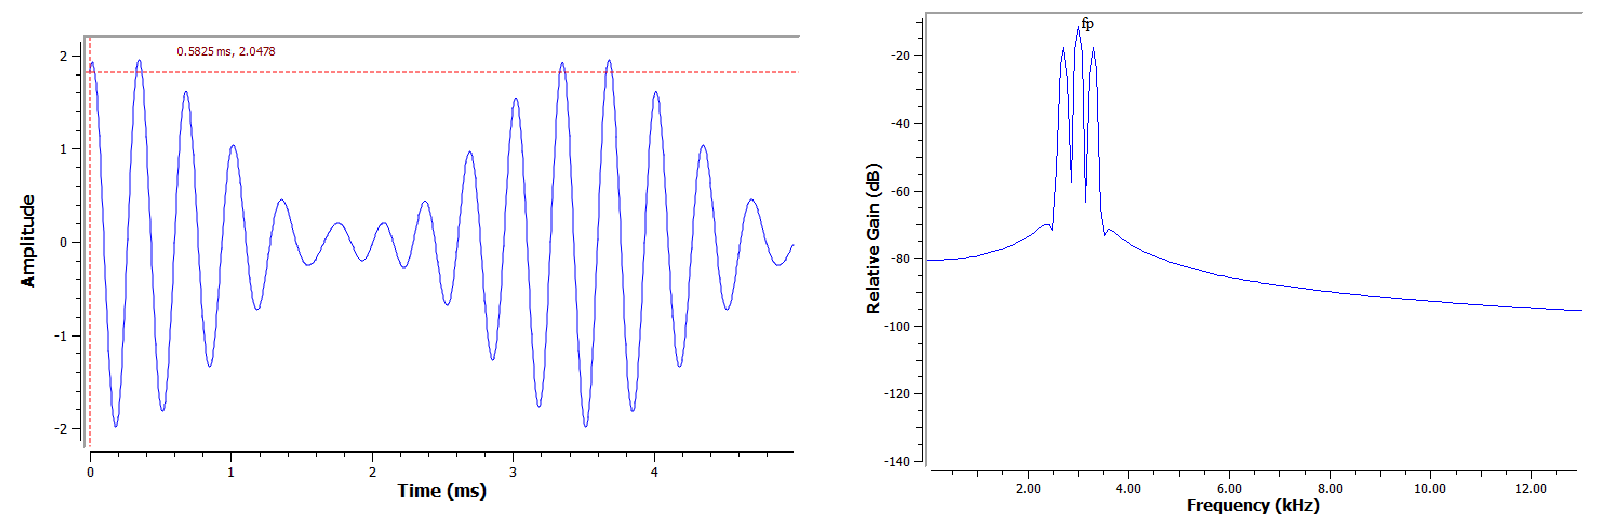
\includegraphics[width=\linewidth]{ImagenesEjercicio8/input}
	\caption{Señal original}
	\label{fig:input}
\end{figure}
En la figura \ref{fig:input} podemos observar la señal $AM$ tanto en el dominio del tiempo como en la frecuencia donde se están presentes la señal portadora (lóbulo central) y la moduladora en los lóbulos laterales.

Debajo se encuentran las imagenes obtenidas mediante $LTSpice$
\begin{figure}[H]
	\centering
	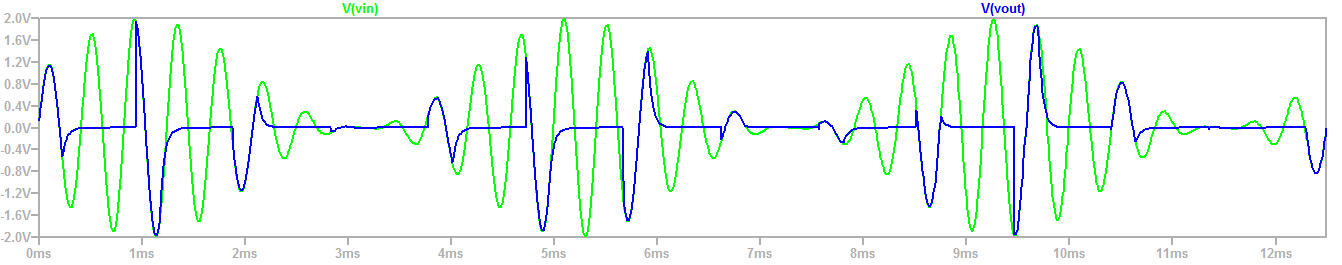
\includegraphics[width=\linewidth]{ImagenesEjercicio8/MuestreoNatural1056time.png}
	\caption{}
	\label{fig:muestreonatural1056time}
\end{figure}
\begin{figure}[H]
	\centering
	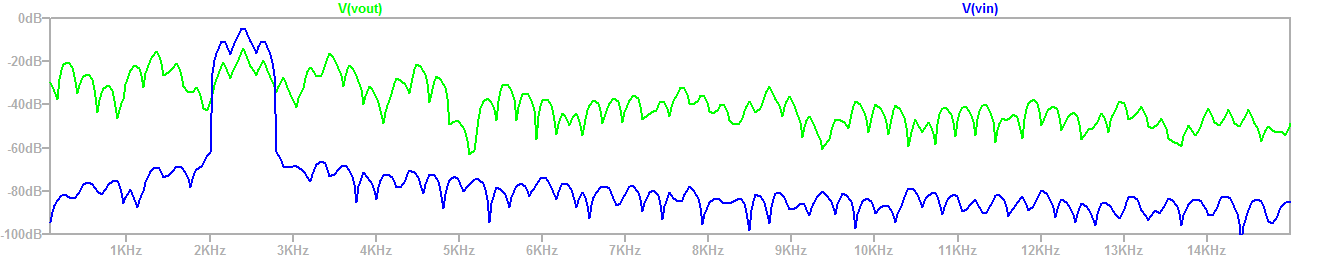
\includegraphics[width=\linewidth]{ImagenesEjercicio8/FFT1056_MuestreoNatural.png}
	\caption{FFT de la señal muestreada a 1056 muestras por segundo}
	\label{fig:FFT_muestreonatural1056time}
\end{figure}
Como se puede apreciar en la figura \ref{fig:FFT_muestreonatural1056time} se ha conservado el espectro y este ha sido trasladado a un espacio espectral por debajo de $1KHz$, además como se utilizo $m=4$(es decir un valor \textbf{par}) no hay inversión espectral en los espectros de numeración impar

A continuación las imágenes obtenidas mediante nuestro entorno de simulación
\begin{figure}[H]
	\centering
	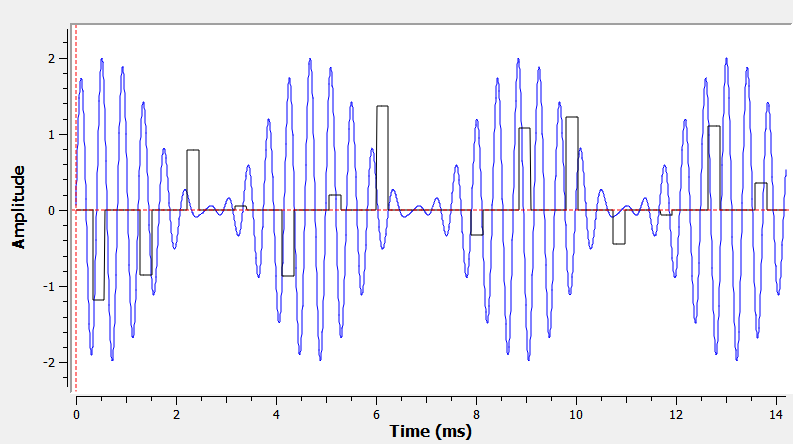
\includegraphics[width=\linewidth]{ImagenesEjercicio8/MuestreoNatural1056timeGNURADIO.png}
	\caption{Señal muestreada a 1056 muestras por segundo en el entorno de simulación}
	\label{fig:AMmuestreonatural1056timeGNU}
\end{figure}
\begin{figure}[H]
	\centering
	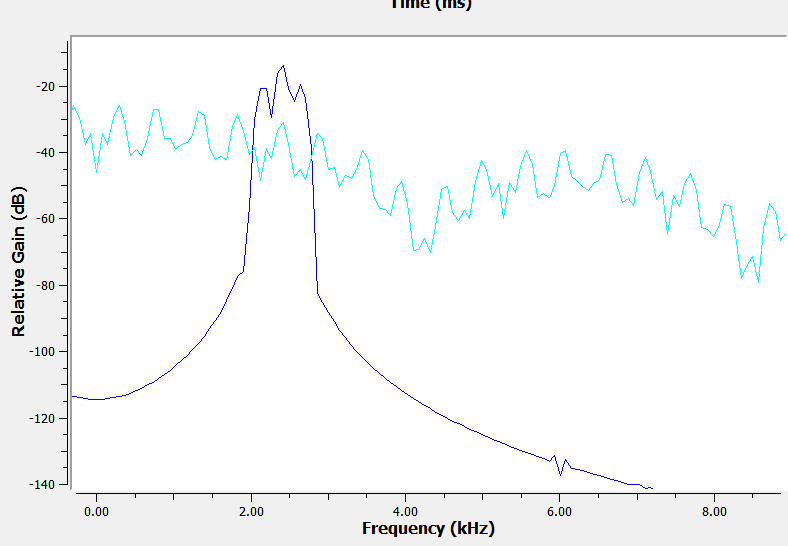
\includegraphics[width=\linewidth]{ImagenesEjercicio8/FFT1056_MuestreoNaturalGNURADIO.png}
	\caption{FFT de la señal muestreada a 1056 muestras por segundo en el entorno de simulación}
	\label{fig:FFT_muestreonatural1056timeGNU}
\end{figure}


Nuevamente se utilizo $LTSpice$ para simular la utilización del modulo \textit{Sample and Hold}

\begin{figure}[H]
	\centering
	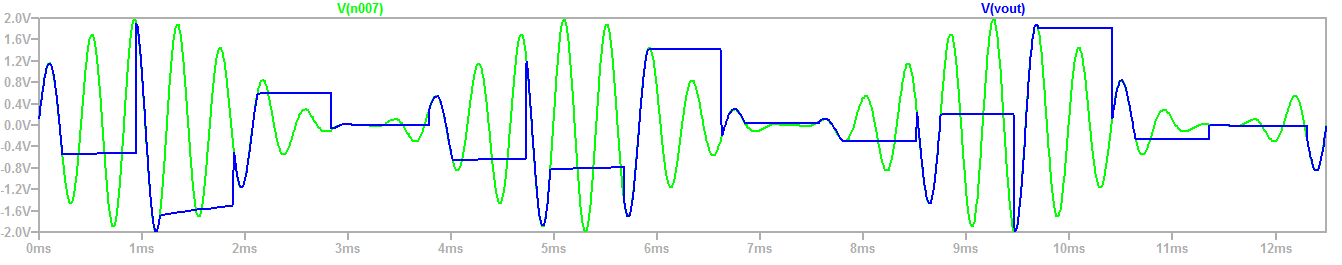
\includegraphics[width=\linewidth]{ImagenesEjercicio8/MuestreoSH1056time}
	\caption{Señal de AM muestreada con Sample and Hold}
	\label{fig:muestreosh1056time}
\end{figure}

\begin{figure}[H]
	\centering
	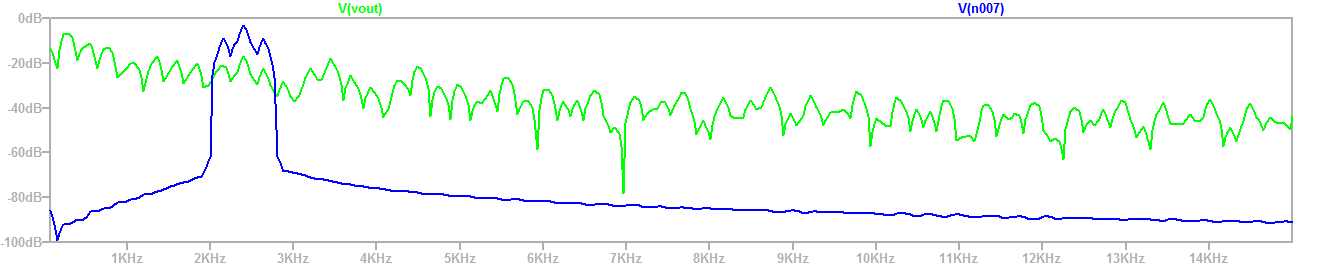
\includegraphics[width=\linewidth]{ImagenesEjercicio8/FFT1056_SampleHold}
	\caption{FFT de la señal de AM muestreada a 1056 muestras por segundo}
	\label{fig:fft1056samplehold}
\end{figure}
En esta ocasión podemos observar un espectro mucho más propenso a sufrir de aliasing. 

\begin{figure}[H]
	\centering
	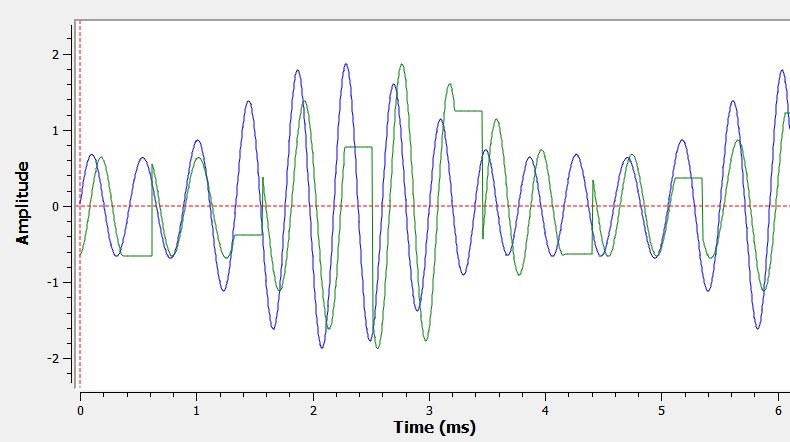
\includegraphics[width=\linewidth]{ImagenesEjercicio8/Muestreo_SH_1056timeGNURADIO}
	\caption{Sample and Hold simulado en el entorno de simulación}
	\label{fig:muestreosh1056timegnuradio}
\end{figure}

\begin{figure}[H]
	
	\centering
	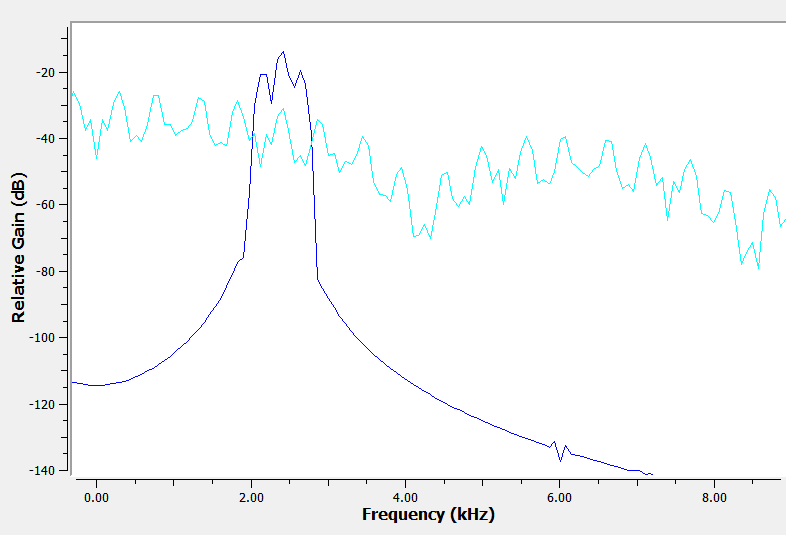
\includegraphics[width=\linewidth]{ImagenesEjercicio8/FFT1056_SH_GNURADIO}
	\caption{FFT de la señal luego del Samplen and Hold a 1056 muestras por segundo en el entorno de simulación}
	\label{fig:fft1056shgnuradio}
\end{figure}

Podemos concluir que la utilización cuidadosa del método de sub-muestreo facilita el diseño de sistemas para que estos trabajen a frecuencias menores, además permite ahorrar el costo de circuitos analógicos que trasladan las señales de interés a frecuencias menores en equipos de radio.

 al mismo tiempo que practica la economía de ancho de banda, un recurso limitado a la hora de transmitir información.

Por último, recomendamos la lectura de \textit{Application Report Why use Oversampling when Undersampling can do the Job?
} de Texas Instruments.

%\end{document}